\documentclass[aps, 10pt, english, twoside, pra, nofootinbib, longbibliography]{revtex4-1}

\usepackage{shared}
% \usepackage{xparse}
\usepackage{cleveref}

% % === Required for matplotlib2tikz ===
% \usepackage[utf8]{inputenc}
% % \usepackage{fontspec}
% \usepackage{pgfplots}

% \usepackage{pgf}

% === Drafting Declarations ===
\draftprofile[TC Fraser]{TC}{Red}
\draftprofile[Elie Wolfe]{E}{Green}

\theoremstyle{plain}
\newtheorem{theorem}{Theorem}
\newtheorem{lemma}[theorem]{Lemma}

\theoremstyle{definition}
\newtheorem{definition}[theorem]{Definition}
\newtheorem{example}[theorem]{Example}

\theoremstyle{remark}
\newtheorem{remark}[theorem]{Remark}

\newcommand{\hgraph}{\mathcal{H}}
\newcommand{\graph}{\mathcal{G}}
\newcommand{\nodes}{\mathcal{N}}
\newcommand{\weights}{\mathcal{W}}
\newcommand{\edges}{\mathcal{E}}
\newcommand{\trans}{\mathcal{T}}
\newcommand{\ind}{\mathcal{I}}
\newcommand{\perm}{\Omega}
\newcommand{\Hilb}{\mathcal{H}}

\newcommand{\ancestralindep}{\perp}

\newcommand{\setoperator}[1]{%
\expandafter\DeclareDocumentCommand\csname#1\endcsname{O{} O{} m}{{\text{#1}_{##1}^{##2}\!}\br{##3}}%
}

\setoperator{Pa}
\setoperator{Ch}
\setoperator{An}
\setoperator{Sub}
\setoperator{AnSub}
\setoperator{Ext}
\setoperator{Com}
% \newcommand{\Pa}[2][]{{\mathsf{Pa}_{#1}\!}\br{#2}}

\newcommand{\term}[1]{\textcolor{Mahogany}{\textbf{#1}}}
\newcommand{\outc}[1]{o\!\bs{#1}}
\DeclareDocumentCommand{\prob}{O{} O{}}{\ifthenelse{\equal{#1}{}}{P}{P_{#1}}\ifthenelse{\equal{#2}{}}{}{\!\br{#2}}}
\DeclareDocumentCommand{\probvec}{O{} O{}}{\ifthenelse{\equal{#1}{}}{\mathcal{P}}{\mathcal{P}_{#1}}\ifthenelse{\equal{#2}{}}{}{\!\br{#2}}}

\usepackage{kbordermatrix}
\renewcommand{\kbldelim}{(}% Left delimiter
\renewcommand{\kbrdelim}{)}% Right delimiter
% \setlength{\parindent}{0pt}

\begin{document}
    \title{Inequalities Witnessing Quantum Incompatibility in The Triangle Scenario}
    \author{Thomas C. Fraser}
    \email{tcfraser@tcfraser.com}
    \affiliation{Perimeter Institute for Theoretical Physics, Waterloo, Ontario, Canada \\ University of Waterloo, Waterloo, Ontario, Canada}
    \date{\today}
    \begin{abstract}
        This document is my current working draft of a paper to do with causal inference, inflation, incompatibility inequalities, hypergraph transversals and quantum correlations.
    \end{abstract}
    \maketitle

    \section{Introduction}
    \section{Definitions \& Notation}

    \begin{definition}
        Borrowing the notation from \cite{Fritz_2014}, each random variable $v$ has a set of all possible outcomes called the \term{outcome space} or \term{valuation space} and is denoted $O_v$. When referencing a \textit{specific} element of $O_v$ or \textit{valuation} of $v$, the notation $\outc{v}$ is used. This notation generalizes to set of random variables $V = \bc{v_1, \ldots, v_{\abs{V}}}$;
        a specific outcome of $\outc{V} \in O_V$ is used to reference a particular tuple or vector of outcomes,
        \[ \outc{V} \defined \br{\outc{v_1}, \outc{v_2}, \ldots, \outc{v_{\abs{V}}} } = \br{\outc{v}}_{v \in V} \eq \label{eq:outcomespace}\]
        It is important to note that the ordering of events in \cref{eq:outcomespace} is irrelevant. Similarly, the outcome space $O_V$ for a set of random variables $V$ is the \term{valuation product} of the individual outcome spaces,
        \[ O_V \defined O_{v_1} \times \cdots \times O_{v_{\abs{V}}} \]
        Where `$\times$' denotes is defined such that,
        \[ \outc{A} \times \outc{B} \defined \br{\outc{a_1}, \ldots, \outc{a_{\abs{A}}}, \outc{b_1}, \ldots, \outc{b_{\abs{B}}}} \]
        When referencing the probability that and set of variables $V$ has outcome $\outc{V}$ (say $v_1 = 0, v_2 = 3$), we intend for the following class of notations to be used interchangeably.
        \[ \prob[V][\outc{V}] = \prob[][\outc{V}] = \prob[][\outc{v_1}\outc{v_2}] = \prob[][v_1 = 0, v_2 = 3] = \prob[][v_2 = 3, v_1 = 0] = \prob[v_1, v_2][03] \]
    \end{definition}

    \begin{definition}
        \label{def:extendable}
        An outcome $\outc{V}$ is said to be \term{extendable} to an outcome $\outc{W}$ (where $V \subseteq W$) if there exists an outcome $\outc{W\setminus V}$ such that $\outc{W} = \outc{W\setminus V} \times \outc{V}$.
        \[ \Ext{\outc{V} \to \outc{W}} \iff \exists \outc{W\setminus V} \mid \outc{W} = \outc{W\setminus V} \times \outc{V} \]
        The idea being that a \textit{less specific} outcome $\outc{V}$ can be made \textit{more specific} by assigning outcomes to the remaining random variables in $W \setminus V$. If such an outcome $\outc{W\setminus V}$ exists, it is unique.
    \end{definition}

    \begin{definition}
        The set of all extendable outcomes of $\outc{V}$ in $O_{W}$ is called the \term{extendable set} and can be written as,
        \[ \Ext[W]{\outc{V}} \defined \outc{V} \times O_{W\setminus V} \defined \bc{\outc{W} \in O_{W} \mid \Ext{\outc{V} \to \outc{W}}} \]
        The extendable set of $\outc{V}$ in $W$ is the set of all outcomes of $O_W$ that \textit{agree} with $\outc{V}$ about valuations for variables in $V$. In this language, two outcomes $\outc{V}$ and $\outc{W}$ are \term{compatible} if they are both extendable to some outcome $\outc{V \cup W}$. Equivalently, $\outc{V}$ and $\outc{W}$ agree on their valuations of $V \cap W$.
        \[ \Com{\outc{V}, \outc{W}} \iff \exists \outc{V \cup W} \mid \Ext{\outc{V} \to \outc{V \cup W}}, \Ext{\outc{W} \to \outc{V \cup W}} \]
    \end{definition}

    \begin{example}
        Consider two sets of random variables $V = \bc{a, b}$ and $W = \bc{a, b, c}$. Clearly $V \subseteq W$; a prerequisite for extendability. Also take all individual outcome spaces to be finite and of order 3: $O_a = O_b = O_c = \bc{1,2,3}$. Then $\outc{V} = \outc{\bc{a,b}} = \br{a = 1, b = 2}$ is extendable to the outcome $\outc{W} = \br{a = 1, b = 2, c = 1}$, and the extendable set of $\outc{V}$ in $O_{W}$ is,
        \[ \Ext[a,b,c]{a = 1, b = 2} = \bc{\br{a = 1, b = 2, c = 1}, \br{a = 1, b = 2, c = 2}, \br{a = 1, b = 2, c = 3}} \]
    \end{example}

    % \begin{definition}
    %     Two outcomes $\outc{V_1}$ and $\outc{V_2}$ over two distinct sets of random variables $V_1$ and $V_2$ are called \term{accordant} or \textit{compatible} if they are mutually realizable. In terms of extendable sets, $\outc{V_1}$ and $\outc{V_2}$ are accordant if there exists an outcome $\outc{V_1 \cup V_2} \in O_{V_1 \cup V_2}$ such that,
    %     \[ \outc{V_1}, \outc{V_2} \subseteq \outc{V_1 \cup V_2}  \]
    %     Accordance between two outcomes is the \textit{opposite} of exclusive.
    % \end{definition}

    \begin{definition}
        \label{def:graph}
        A \term{graph} is an ordered tuple $\br{\nodes, \edges}$ of \textit{nodes} and \textit{edges} respectively where the nodes can represent any object and the edges are pairs of nodes. For convenience of notation, one defines an index set over the nodes denoted $\ind_\nodes$.
        \[ \nodes = \bc{n_i \mid i \in \ind_\nodes} \quad \edges = \bc{\bc{n_j, n_k} \mid j,k \in \ind_\nodes} \]
    \end{definition}

    \begin{definition}
        \label{def:directed_graph}
        A \term{directed graph} $\graph$ is an ordered tuple $\br{\nodes, \edges}$ of \textit{nodes} and \textit{edges} respectively where the nodes can represent any object and the edges are \textit{ordered} pairs of nodes. For convenience of notation, one defines an index set over the nodes denoted $\ind_\nodes$.
        \[ \nodes = \bc{n_i \mid i \in \ind_\nodes} \quad \edges = \bc{n_j \to n_k \mid j,k \in \ind_\nodes} \]
    \end{definition}

    \begin{definition}
        \label{def:graph_terms}
        The following definitions are common language in directed graph theory. Let $n, m \in \nodes$ be example nodes of the graph $\graph$.
        \begin{itemize}
            \item The \term{parents of a node}: $\Pa[\graph]{n} \defined \bc{m \mid m \to n}$
            \item The \term{children of a node}: $\Ch[\graph]{n} \defined \bc{m \mid n \to m}$
            \item The \term{ancestry of a node}: $\An[\graph]{n} \defined \bigcup_{i\in\mathbb{W}} \Pa[\graph][i]{n}$ where $\Pa[\graph][i]{n} \defined \Pa[\graph]{\Pa[\graph][i-1]{n}}$ and $\Pa[\graph][0]{n} = n$
        \end{itemize}
        All of these terms can be generalized to sets of nodes $N \subseteq \nodes$ through union over the elements,
        \begin{itemize}
            \item The \term{parents of a node set}: $\Pa[\graph]{N} \defined \bigcup_{n\in N}\Pa[\graph]{n}$
            \item The \term{children of a node set}: $\Ch[\graph]{N} \defined \bigcup_{n\in N}\Ch[\graph]{n}$
            \item The \term{ancestry of a node set}: $\An[\graph]{N} \defined \bigcup_{n\in N}\An[\graph]{n}$
        \end{itemize}
        Moreover, an \term{induced subgraph} of $\graph$ due to a set of nodes $N \subseteq \nodes$ is the graph composed of $N$ and all edges $e \in \edges$ of the original graph that are contained in $N$.
        \[ \Sub[\graph]{N} \defined \br{N, \bc{e_i \mid i \in \ind_\edges, e_i \subseteq N}}\]
        An \term{ancestral subgraph} of $\graph$ due to $N \subseteq \nodes$ is the induced subgraph due to the ancestry of $N$.
        \[ \AnSub[\graph]{N} \defined \Sub[\graph]{\An[\graph]{N}} \]
    \end{definition}

    \begin{definition}
        \label{def:dag}
        A \term{directed acyclic graph} or \term{DAG} $\graph$ is an directed graph \cref{def:directed_graph} with the additional property that no node $n$ is in its set of \term{ancestors}.
        \[ \forall n \in \nodes : n \notin \bigcup_{i\in\mathbb{N}} \Pa[\graph][i]{n}\]
        Notice the difference between using the natural numbers $\mathbb{N}$ to distinguish \textit{ancestors} from \textit{ancestry}.
    \end{definition}

    \begin{definition}
        \label{def:hypergraph}
        A \term{hypergraph} denoted $\hgraph$ is an ordered tuple $\br{\nodes, \edges}$ of \textit{nodes} and \textit{edges} respectively where the nodes can represent any object and the edges are \textit{subsets} of nodes. For convenience of notation, one defines an index set over the nodes and edges of a hypergraph $\hgraph$ denoted $\ind_\nodes$ and $\ind_\edges$ respectively.
        \[ \hgraph = \br{\nodes, \edges} \quad \nodes = \bc{n_i \mid i \in \ind_\nodes} \quad \edges = \bc{e_i \mid i \in \ind_\edges, e_i \subseteq \nodes} \]
        Note that whenever the index for an edge or node is arbitrary, it will be omitted. There is a dual correspondence between edges $e \in \edges$ and nodes $n \in \nodes$ in a Hypergraph. An edge $e$ is viewed as a set of nodes $\bc{n_i}$, and a node $n$ can be viewed as the set of edges $\bc{e_i}$ that contain it.
    \end{definition}

    \begin{definition}
        \label{def:hgraph_trans}
        A \term{hypergraph transversal} (or edge hitting set) $\trans$ of a hypergraph $\hgraph$ is a set of nodes $\trans \subseteq \nodes$ that have non-empty intersections with every edge in $\edges$.
        \[ \trans = \bc{n_i \in \nodes \mid i \in \ind_\trans } \quad \forall e \in \edges : \trans \cap e \neq \emptyset \]
    \end{definition}

    \begin{definition}
        A \term{minimal hypergraph transversal} $\trans$ is any valid transversal (\cref{def:hgraph_trans}) of $\hgraph$ where every node $n$ is \textit{necessary} to retain validity. For each node $n$ in $\trans$, $\trans \setminus n$ is no longer a transversal.
        \[ \trans = \bc{n_i \in \nodes \mid i \in \ind_\trans } \quad \forall i \in \ind_\trans, \exists e \in \edges : \br{\trans \setminus n_i} \cap e = \emptyset \]
    \end{definition}

    \begin{definition}
        A \term{weighted hypergraph} $\hgraph_\weights$ is a regular hypergraph satisfying \cref{def:hypergraph} equipped with a set of weights $\weights$ ascribed to each node such that a weighted hypergraph is written as a triplet $\br{\weights, \nodes, \edges}$.
        \[ \weights = \bc{w_i \mid i \in \ind_\nodes, w_i \in \R} \]
        One would say that a particular node $n_i$ carries weight $w_i$ for each $i \in \ind_\nodes$.
    \end{definition}

    \begin{definition}
        A \term{bounded transversal} of a weighted hypergraph $\hgraph_\weights$ is a transversal $\trans$ of the unweighted hypergraph $\hgraph$ and a real number $t$ (denoted $\trans_{\leq t}$) such that the sum of the node weights of the transversal is bounded by $t$.
        \[ \trans_{\leq t} = \bc{n_i \mid i \in \ind_\trans} \quad \text{s.t.} \sum_{j\in\ind_\trans} w_j \leq t \]
        One can definte analogous \term{(strictly) upper/lower bounded transversals} by considering modifications of the notation: $\trans_{< t}, \trans_{\geq t}, \trans_{> t}$.
    \end{definition}

    \begin{definition}
        A \term{causal structure} is simply a DAG with the extra classification of each node into one of two categories; the \term{latent nodes} and \term{observed nodes} denoted $\nodes_L$ and $\nodes_O$. The latent nodes correspond to random variables that are either hidden through some fundamental process or cannot/will not be measured. The observed nodes are random variables that are measurable. Every node is either latent or observed and no node is both:
        \[ \nodes_L \cap \nodes_O = \emptyset \qquad \nodes_L \cup \nodes_O = \nodes \]
    \end{definition}

    \begin{definition}
        The \term{product distribution} two distributions is denoted as usual with $\times$ and is defined as,
        \[ \br{\prob[v] \times \prob[w]}\br{\outc{v}, \outc{w}} \defined \prob[v][\outc{v}]\prob[w][\outc{w}] \]
        A product distribution of $k$ distributions is defined recursively,
        \[ \prod_{i=1}^{k} \prob[v_i] \defined \br{\prob[v_1] \times \cdots \times \prob[v_k]} \]
    \end{definition}

    \begin{definition}
        The \term{marginalization} of a distribution $\prob[v \cup w]$ to the distribution $\prob[v]$ is denoted $\sum_{w} \prob[v \cup w] = \prob[v]$ and is defined such that,
        \[ \forall \outc{v} \in O_v : \br{\sum_{w} \prob[v, w]}\br{\outc{v}} \defined \sum_{o\bs{w} \in O_w} \prob[v, w][\outc{v}, \outc{w}] \]
    \end{definition}

    \todo[TC]{How many definitions do I need to write??}

    \section{Triangle Scenario}
    \todo[TC]{Discuss the Triangle Scenario, previous work done on it, etc.}
    Focusing on the inflation depicted in \cref{fig:inflated_triangle_scenario}, we obtained the maximally pre-injectable sets through the procedure outlined in \cite{Inflation}.
    \begin{equation}
        \begin{gathered}
            \textbf{Maximal Pre-injectable Sets $\Pi$} \\
            \bc{A_1, B_1, C_1, A_4, B_4, C_4} \\
            \bc{A_1, B_2, C_3, A_4, B_3, C_2} \\
            \bc{A_2, B_3, C_1, A_3, B_2, C_4} \\
            \bc{A_2, B_4, C_3, A_3, B_1, C_2} \\
            \bc{A_1, B_3, C_4} \\
            \bc{A_1, B_4, C_2} \\
            \bc{A_2, B_1, C_4} \\
            \bc{A_2, B_2, C_2} \\
            \bc{A_3, B_3, C_3} \\
            \bc{A_3, B_4, C_1} \\
            \bc{A_4, B_1, C_3} \\
            \bc{A_4, B_2, C_1}
        \end{gathered}
        \qquad
        \begin{gathered}
            \textbf{Ancestral Independences} \\
            \bc{A_1, B_1, C_1} \ancestralindep \bc{A_4, B_4, C_4} \\
            \bc{A_1, B_2, C_3} \ancestralindep \bc{A_4, B_3, C_2} \\
            \bc{A_2, B_3, C_1} \ancestralindep \bc{A_3, B_2, C_4} \\
            \bc{A_2, B_4, C_3} \ancestralindep \bc{A_3, B_1, C_2} \\
            \bc{A_1} \ancestralindep \bc{B_3} \ancestralindep \bc{C_4} \\
            \bc{A_1} \ancestralindep \bc{B_4} \ancestralindep \bc{C_2} \\
            \bc{A_2} \ancestralindep \bc{B_1} \ancestralindep \bc{C_4} \\
            \bc{A_2} \ancestralindep \bc{B_2} \ancestralindep \bc{C_2} \\
            \bc{A_3} \ancestralindep \bc{B_3} \ancestralindep \bc{C_3} \\
            \bc{A_3} \ancestralindep \bc{B_4} \ancestralindep \bc{C_1} \\
            \bc{A_4} \ancestralindep \bc{B_1} \ancestralindep \bc{C_3} \\
            \bc{A_4} \ancestralindep \bc{B_2} \ancestralindep \bc{C_1}
        \end{gathered}
    \end{equation}
    As can be counted, there are $12$ maximally pre-injectable sets which will be indexed $1$ through $12$ in the order seen above ($\Pi = \bc{\Pi_1, \ldots, \Pi_{12}}$)

    % =========================
    % Causal Structure Diagrams
    % =========================
    \definecolor{obs_outline}{RGB}{51,157,215}
    \definecolor{obs_fill}{RGB}{222,253,255}
    \definecolor{obs_text}{RGB}{0,0,0}
    \definecolor{lat_outline}{RGB}{251,141,54}
    \definecolor{cause}{RGB}{30, 0, 30}
    \definecolor{lat_fill}{RGB}{255,213,153}
    \definecolor{lat_text}{RGB}{0,0,0}
    \tikzset{square/.style={regular polygon,regular polygon sides=4}}
    \tikzset{triangle/.style={regular polygon,regular polygon sides=3}}
    \tikzset{observed/.style={obs_text, triangle, thick, draw=obs_outline, fill=obs_fill, inner sep=0em, minimum size=3em}}
    \tikzset{latent/.style={lat_text, circle, thick, draw=lat_outline, fill=lat_fill}}
    % \tikzset{cause/.style={mid arrow/.style={postaction={decorate,decoration={markings, mark=at position .5 with {\arrow[#1]{stealth}}}}},}}
    \tikzset{
      % style to apply some styles to each segment of a path
      on each segment/.style={
        decorate,
        decoration={
          show path construction,
          moveto code={},
          lineto code={
            \path [#1]
            (\tikzinputsegmentfirst) -- (\tikzinputsegmentlast);
          },
          curveto code={
            \path [#1] (\tikzinputsegmentfirst)
            .. controls
            (\tikzinputsegmentsupporta) and (\tikzinputsegmentsupportb)
            ..
            (\tikzinputsegmentlast);
          },
          closepath code={
            \path [#1]
            (\tikzinputsegmentfirst) -- (\tikzinputsegmentlast);
          },
        },
      },
      % style to add an arrow in the middle of a path
      mid arrow/.style={postaction={decorate,decoration={
            markings,
            mark=at position .6 with {\arrow[scale=1.5, cause]{stealth}}
          }}},
    }
    \begin{figure}
    \begin{center}
        \begin{minipage}[b]{.48\textwidth}
            \centering
            \scalebox{1.0}{%
            \begin{tikzpicture}[scale=1]
                \begin{scope}[every node/.style=observed]
                    \node (C) at (-2, 0) {$C$};
                    \node (B) at (2, 0) {$B$};
                    \node (A) at (0, {2*sqrt(3)}) {$A$};
                \end{scope}
                \begin{scope}[every node/.style=latent]
                    \node (X) at (-1, {sqrt(3)}) {$X$};
                    \node (Y) at (1, {sqrt(3)}) {$Y$};
                    \node (Z) at (0, 0) {$Z$};
                \end{scope}
                \begin{scope}[every path/.style={draw=cause, thick}]
                    \path[postaction={on each segment={mid arrow}}]
                    (X) -- (A)
                    (X) -- (C)
                    (Y) -- (A)
                    (Y) -- (B)
                    (Z) -- (B)
                    (Z) -- (C);
                \end{scope}
            \end{tikzpicture}
            }
            \caption{The casual structure of the Triangle Scenario. Three variables $A,B,C$ are observable and illustrated as triangles, while $X, Y, Z$ are latent variables illustrated as circles.}
            \label{fig:triangle_scenario}
        \end{minipage}\hspace{0.04\textwidth}%
        \begin{minipage}[b]{.48\textwidth}
            \centering
            \scalebox{0.8}{%
            \newcommand{\ift}{2.3}
            \begin{tikzpicture}[scale=2]
                \begin{scope}[every node/.style=observed]
                    \node (C4) at (-2, 0) {$C_4$};
                    \node (C3) at ({-2 + 1/\ift}, {1/(\ift*sqrt(3))}) {$C_3$};
                    \node (C2) at ({-2 + 2*1/\ift}, {2*1/(\ift*sqrt(3))}) {$C_2$};
                    \node (C1) at ({-2 + 3*1/\ift}, {3*1/(\ift*sqrt(3))}) {$C_1$};
                    \node (B4) at (2, 0) {$B_4$};
                    \node (B3) at ({2 - 1/\ift}, {1/(\ift*sqrt(3))}) {$B_3$};
                    \node (B2) at ({2 - 2*1/\ift}, {2*1/(\ift*sqrt(3))}) {$B_2$};
                    \node (B1) at ({2 - 3*1/\ift}, {3*1/(\ift*sqrt(3))}) {$B_1$};
                    \node (A4) at (0, {2*sqrt(3)}) {$A_4$};
                    \node (A3) at (0, {2*sqrt(3) - 2/sqrt(3)*(1/\ift)}) {$A_3$};
                    \node (A2) at (0, {2*sqrt(3) - 2*2/sqrt(3)*(1/\ift)}) {$A_2$};
                    \node (A1) at (0, {2*sqrt(3) - 3*2/sqrt(3)*(1/\ift)}) {$A_1$};
                \end{scope}
                \begin{scope}[every node/.style=latent]
                    \node (X2) at (-1, {sqrt(3)}) {$X_2$};
                    \node (X1) at ({-1 + 1/\ift}, {sqrt(3) - 1/(\ift*sqrt(3))}) {$X_1$};
                    \node (Y2) at (1, {sqrt(3)}) {$Y_2$};
                    \node (Y1) at ({1 - 1/\ift}, {sqrt(3) - 1/(\ift*sqrt(3))}) {$Y_1$};
                    \node (Z1) at (0, 0.5) {$Z_1$};
                    \node (Z2) at (0, 0) {$Z_2$};
                \end{scope}
                \begin{scope}[every path/.style={draw=cause, thick}]
                    \path[postaction={on each segment={mid arrow}}]
                    (X2) -- (A4) (X2) -- (C4) (X2) -- (C2) (X2) -- (A3)
                    (Y2) -- (A4) (Y2) -- (B4) (Y2) -- (A2) (Y2) -- (B3)
                    (Z2) -- (B4) (Z2) -- (C4) (Z2) -- (B2) (Z2) -- (C3)
                    (X1) -- (A1) (X1) -- (C1) (X1) -- (C3) (X1) -- (A2)
                    (Y1) -- (A1) (Y1) -- (B1) (Y1) -- (A3) (Y1) -- (B2)
                    (Z1) -- (B1) (Z1) -- (C1) (Z1) -- (B3) (Z1) -- (C2)
                    ;
                \end{scope}
            \end{tikzpicture}
            }
            \caption{An inflated causal structure of the Triangle Scenario \cref{fig:triangle_scenario}.}
            \label{fig:inflated_triangle_scenario}
        \end{minipage}
    \end{center}
    \end{figure}
    % =========================
    % =========================

    \section{Summary of the Inflation Technique}
    The causal inflation technique, first pioneered by Wolfe, Spekkens, and Fritz \cite{Inflation} and inspired by the \textit{do calculus} and \textit{twin networks} of Ref. \cite{Pearl_2009}, is a family of causal inference techniques that can be used to determine if a probability distribution is compatible or incompatible with a given causal structure. As a preliminary summary, the inflation technique begins by \textit{augmenting} a causal structure with additional nodes, producing the \textit{inflated} causal structure, and then exposes how causal inference tasks on the inflated causal structure can be used to make inferences on the original causal structure. Equipped with the common graph-theoretic terminology and notation of \cref{def:graph_terms}, an inflation can be formally defined as follows:
    \begin{definition}
        An \term{inflation} of a causal structure $\graph$ is another causal structure $\graph'$ such that:
        \[ \forall n' \in \nodes' : \AnSub[\graph']{n'} \sim \AnSub[\graph]{n} \]
        Where `$\sim$' is notation for equivalence up to removal of the copy-index. To clarify, each node in an inflated causal structure $n' \in \nodes'$ shares a \textit{label} assigned to a node $n \in \nodes$ in the original causal structure together with an additional index called the \term{copy-index}.
    \end{definition}
    \begin{definition}
        A set of \term{causal parameters} for a particular causal structure $\graph$ is the specification of a conditional distribution for every node $n \in \nodes$ given it's parents in $\graph$.
        \[ \bc{\prob[n \mid \Pa[\graph]{n}] \mid n \in \nodes} \]
    \end{definition}
    \todo[TC]{Clean up what is meant by copy index, example maybe?}
    \todo[TC]{Define injectable sets}
    \todo[TC]{Define pre-injectable sets and then it's connection to probabilities}
    \todo[TC]{Define pre-injectable sets}
    \todo[TC]{State the main Compatibility lemma of inflation}
    \section{Compatibility, Contextuality and the Marginal Problem}
    In order to determine if a given marginal distribution $\prob[V]$ or set of marginal distributions $\bc{\prob[V_1], \ldots, \prob[V_k]}$ is compatible with a causal structure $\graph$, one should first formalize what is meant by \textit{compatible}.
    \begin{definition}
        \label{def:compatible}
        A marginal distribution $\prob[V]$ is \term{compatible} with a causal structure $\graph$ (where it is assumed that $V \subseteq \nodes_O$) if there exists a \textit{choice} of causal parameters $\bc{\prob[n \mid \Pa[\graph]{n}] \mid n \in \nodes}$ such that $\prob[V]$ can be \textit{recovered} from the following series of operations:

        \todo[TC]{Define this notation here}
        \begin{enumerate}
            \item First obtain a joint distribution over \textit{all} nodes of of the causal structure,
            \[ \prob[\nodes] = \prod_{n \in \nodes} \prob[n \mid \Pa[\graph]{n}] \]
            \item Then marginalize over the latent nodes of $\graph$,
            \[ \prob[\nodes_O] = \sum_{\nodes_L} \prob[\nodes] \]
            \item Finally marginalize over the observed nodes not in $V$ to obtain $\prob[V]$,
            \[ \prob[V] = \sum_{\nodes_O \setminus V} \prob[\nodes_O] \]
        \end{enumerate}
        A set of marginal distributions $\bc{\prob[V_1], \ldots, \prob[V_k]}$ is compatible with $\graph$ if each of the distributions can be made compatible by the \textit{same} choice of causal parameters.
        A distribution $\prob[V]$ or set of distributions $\bc{\prob[V_1], \ldots, \prob[V_k]}$ is said to be \term{incompatible} with a causal structure if there \textit{does not exist} a set of causal parameters with the above mentioned property.

        \todo[TC]{Source this?}
    \end{definition}

    Operations 2 and 3 of \cref{def:compatible} are related to the \textit{marginal problem}.
    \begin{definition}
        \label{def:marginal_problem}
        \term{The Marginal Problem:} Given a set of distributions $\bc{\prob[V_1], \ldots, \prob[V_k]}$ where $V_i \subseteq \mathcal{V}$ for some set of random variables $\mathcal{V}$ and $k \geq 2$, does there exist a joint distribution $\prob[\mathcal{V}]$ such that each given distribution $\prob[V_i]$ can be obtained from marginalizing $\prob[\mathcal{V}]$?
        \[ \forall i \in \bc{1, \ldots, k} : \prob[V_i] = \sum_{\mathcal{V} \setminus V_i} \prob[\mathcal{V}] \]
        Typically (although not strictly necessary), $\mathcal{V}$ is taken to mean the union of all $V_i$'s.
        \[ \mathcal{V} = V_1 \cup \cdots \cup V_k = \bigcup_{i=1}^{k} V_i \eq \label{eq:marginals_union} \]
    \end{definition}

    \begin{definition}
        \label{def:marginal_model}
        A reoccurring motif of these discussions will be the set of distributions $\bc{\prob[V_1], \ldots, \prob[V_k]}$ mentioned in \cref{def:marginal_model}. In agreement with \cite{Fritz_2011} we will call this set of distributions a \term{marginal model} and denote it $\prob^\mathcal{M}$ provided that they are \textit{compatible}:
        \[ \forall i \neq j \text{ if } V_i \cap V_j \neq \emptyset \text{ then } \sum_{V_i \setminus V_j} \prob[V_i] = \sum_{V_j \setminus V_i} \prob[V_j]  \]
        We call the set of subsets $\bc{V_1, \ldots, V_k}$ the marginal contexts or the \term{maximal marginal scenario} \todo[TC]{Clarify maximal} and an individual $V_i$ a \term{marginal context}. Finally we will denote the union of all contexts $\mathcal{V}$ and define it exactly as in \cref{eq:marginals_union}. In addition, we elect to define the \term{marginal outcomes} $O^\mathcal{M}$ to be the set of all outcomes belonging to outcomes of the marginal contexts.
        \[ O^\mathcal{M} \defined O_{V_1} \cup \cdots \cup O_{V_k} = \bigcup_{j=1}^{k} O_{V_j} \]
        Note that $O^\mathcal{M}$ is \textit{not} a valid outcome space, analogous to the fact that $P^\mathcal{M}$ is \textit{not} a probability distribution. Instead $O^\mathcal{M}$ is a collection of outcome spaces just as $P^\mathcal{M}$ is a collection of distributions.
    \end{definition}

    \todo[TC]{Discuss Compatibility, connection to cooperative games/resources, bell incompatibility?}
    \todo[TC]{Connection between contextuality and Compatibility via the marginal problem for causal parameters}
    \todo[TC]{Discuss what is meant by a `complete' solution to the marginal problem}
    \todo[TC]{Maybe define the possibilistic marginal problem for later}
    \section{The Fritz Distribution}
    The \textbf{Fritz distribution} $P_F$ is a quantum-accessible distribution known to be incompatible with the Triangle Scenario. Explicitly, $P_F$ is a three-party ($A,B,C$), four-outcome ($1,2,3,4$) distribution that has form as follows:
    \begin{align*}
    \prob[F][111] = \prob[F][221] = \prob[F][412] = \prob[F][322] = \prob[F][233] = \prob[F][143] = \prob[F][344] = \prob[F][434] &= \f{1}{32}\br{2 + \sqrt{2}} \\
    \prob[F][121] = \prob[F][211] = \prob[F][422] = \prob[F][312] = \prob[F][243] = \prob[F][133] = \prob[F][334] = \prob[F][444] &= \f{1}{32}\br{2 - \sqrt{2}}
    \end{align*}
    Here the notation $\prob[F][abc] = \prob[ABC][abc] = \prob[][A=a,B=b,C=c]$ is used. The Fritz distribution $\prob[F]$ can be realized with the following quantum configuration:
    \begin{gather*}
    \rho_{AB} = \ket{\Psi^+}\bra{\Psi^+} \quad \rho_{BC} = \rho_{CA} = \ket{\Phi^+}\bra{\Phi^+} \\
    M_{A} = \bc{\ket{0\psi_0}\bra{0\psi_0}, \ket{0\psi_{\pi}}\bra{0\psi_{\pi}}, \ket{1\psi_{-\pi/2}}\bra{1\psi_{-\pi/2}}, \ket{1\psi_{\pi/2}}\bra{1\psi_{\pi/2}}} \\
    M_{B} = \bc{\ket{\psi_{\pi/4}0}\bra{\psi_{\pi/4}0}, \ket{\psi_{5\pi/4}0}\bra{\psi_{5\pi/4}0}, \ket{\psi_{3\pi/4}1}\bra{\psi_{3\pi/4}1}, \ket{\psi_{-\pi/4}1}\bra{\psi_{-\pi/4}1}} \\
    M_{C} = \bc{\ket{00}\bra{00}, \ket{01}\bra{01}, \ket{10}\bra{10}, \ket{11}\bra{11}} \\
    \end{gather*}
    Where for convenience of notation $\psi_x$ is used to denote the superposition,
    \[ \ket{\psi_x} = \f{1}{\sqrt{2}}\br{\ket{0} + e^{ix}\ket{1}} \]
    Additionally $\ket{\Psi^+} = \f{1}{\sqrt{2}}\br{\ket{01} + \ket{10}}$ and $\ket{\Phi^+} = \f{1}{\sqrt{2}}\br{\ket{00} + \ket{11}}$ are two maximally entangled Bell states.
    Fritz first proved it's incompatibility \cite{Fritz_2012} by showing $C$ acts a moderator to ensure measurement pseudo-settings for $A$ and $B$ are independent, satisfying non-broadcasting requirements for the standard Bell scenario. In fact, by coarse-graining outcomes for $A$ and $B$ and treating $C$ as a measurement-setting moderator, $P_F$ maximally violates the CHSH inequality. To illustrate this, begin with the CHSH inequality \cite{CHSH_Original},
    \[ \ba{AB|S_A=1, S_B=1} + \ba{AB|S_A=1, S_B=2} + \ba{AB|S_A=2, S_B=1} - \ba{AB|S_A=2, S_B=2} \leq 2 \eq \label{eq:CHSH}\]
    Where $\ba{AB|S_A=i, S_B=j}$ is the correlation between $A$ and $B$ given the measurement settings for $A$ ($B$) is $i$ ($j$) respectively. Next, each of $C$'s outcomes become the condition settings in \cref{eq:CHSH},
    \[ \ba{AB|C=2} + \ba{AB|C=3} + \ba{AB|C=4} - \ba{AB|C=1} \leq 2 \]
    Finally, specifying the correlation between $A$ and $B$ to be defined in terms of a $\bc{1,2,3,4} \rightarrow \bc{\br{1,4}, \br{2,3}}$ coarse-graining,
    \[ \f{\sqrt{2}}{2} + \f{\sqrt{2}}{2} + \f{\sqrt{2}}{2} - \f{-\sqrt{2}}{2} \leq 2 \]
    \[ 2\sqrt{2} \leq 2 \]
    Which corresponds to the maximum quantum violation of the CHSH inequality \cref{eq:CHSH}

    \todo[TC]{Discuss non-uniqueness and relabeling}
    \todo[TC]{Summarize Problem 2.17 in fritz BBT, make it more formal}
    \section{Certificate Inequalities}
    \subsection{Casting the Inflated Marginal Problem as a Linear Program}
    After obtaining the maximal pre-injectable sets associated with a particular inflation, one can write the marginal problem of \cref{def:marginal_problem} as a linear program. The key observation is that marginalization is a \textit{linear} operator that can be performed via a matrix multiplication. To do this, we will define the \textit{marginalization matrix}.
    \begin{definition}
        The \term{marginalization matrix} $M$ for a marginal scenario $\bc{V_1, \dots, V_k}$ is a bit-wise matrix where the columns are indexed by \textit{joint} outcomes $\outc{\mathcal{V}} \in O_{\mathcal{V}}$ and the rows are indexed by \textit{marginal} outcomes corresponding to all outcomes $\outc{V_i} \in O_{V_i} \subseteq O^{\mathcal{M}}$. The entries of $M$ are populated whenever a row index is extendable to a column index.
        \[ M_{\br{o\bs{V_i}, o\bs{\mathcal{V}}}} = \begin{cases}
            1 & \Ext{\outc{V_i} \to \outc{\mathcal{V}}} \\
            0 & \text{otherwise}
        \end{cases} \]
        The marginalization matrix has $\abs{O_\mathcal{V}}$ columns and $\abs{O^{\mathcal{M}}} = \sum_{i=1}^{k} \abs{O_{V_i}}$ rows. The number of non-zero entries of $M$ is a simple expression,
        \[ \sum_{i=1}^{k} \abs{O_{V_i}}\abs{O_{\mathcal{V} \setminus V_i}} = \sum_{i=1}^{k} \abs{O_{\mathcal{V}}} = k\abs{O_{\mathcal{V}}} \]
        Each of the $k$ elements of $\bc{V_1, \ldots, V_k}$ contributes a single non-zero entry to each column of $M$, resulting in $k\abs{O_\mathcal{V}}$ total non-zero entries.

        Note that the row and column indices of the marginalization matrix will be referred to very frequently. We will refer to the
    \end{definition}
    \todo[TC]{Computationally Efficient generation?}

    To illustrate this concretely, consider the following example:
    \begin{example}
        Suppose one has $4$ binary random variables $\mathcal{V} = \bc{a,b,c}$ in mind and $2$ subsets $\bc{\bc{a,c}, \bc{b}}$. Then the marginalization matrix is:
        \[ M = \kbordermatrix{
            (a,b,c) = & (0,0,0) & (0,0,1) & (0,1,0) & (0,1,1) & (1,0,0) & (1,0,1) & (1,1,0) & (1,1,1) \\
            (a=0, c=0) & 1 & 0 & 1 & 0 & 0 & 0 & 0 & 0 \\
            (a=0, c=1) & 0 & 1 & 0 & 1 & 0 & 0 & 0 & 0 \\
            (a=1, c=0) & 0 & 0 & 0 & 0 & 1 & 0 & 1 & 0 \\
            (a=1, c=1) & 0 & 0 & 0 & 0 & 0 & 1 & 0 & 1 \\
            (b=0)      & 1 & 1 & 0 & 0 & 1 & 1 & 0 & 0 \\
            (b=1)      & 0 & 0 & 1 & 1 & 0 & 0 & 1 & 1
        } \]
    \end{example}

    In order to describe how marginalization can be written as matrix multiplication $M \cdot x = b$, we need to describe how to define two more quantities:

    \begin{definition}
        The \term{joint distribution vector} $\probvec[\mathcal{V}]$ for a probability distribution $\prob[\mathcal{V}]$ is the vector whose entries are the positive, real-valued probabilities that $\prob[\mathcal{V}]$ assigns to each outcome of $\outc{\mathcal{V}}$ of $O_\mathcal{V}$. $\probvec[\mathcal{V}]$ shares the same indices as the \textit{column} indices of $M$.
        \[ \probvec[\mathcal{V}]^\intercal = \bs{\prob[\mathcal{V}][\outc{\mathcal{V}}]}_{o\bs{\mathcal{V}} \in O_{\mathcal{V}}} \]
    \end{definition}
    \begin{definition}
        The \term{marginal distribution vector} $\probvec[\bc{V_1, \ldots, V_k}]$ for a marginal model $\bc{P_{V_1}, \ldots, P_{V_k}}$ is the vector whose entries are probabilities over the set of marginal outcomes $O^{\mathcal{M}}$. $\probvec[\bc{V_1, \ldots, V_k}]$ shares the same indices as the \textit{row} indices of $M$.
        \[ \probvec[\bc{V_1, \ldots, V_k}]^\intercal = \bs{\prob[V_i][\outc{V_i}] }_{o\bs{V_i} \in O^{\mathcal{M}}} \]
    \end{definition}
    The marginal and joint distribution vectors are related via the marginalization matrix $M$. Given a joint distribution vector $\probvec[\mathcal{V}]$ one can obtain the marginal distribution vector $\probvec[\bc{V_1, \ldots, V_k}]$ by multiplying $M$ by $\probvec[\mathcal{V}]$.
    \[ \probvec[\bc{V_1, \ldots, V_k}] = M \cdot \probvec[\mathcal{V}] \eq \label{eq:marginal_problem_matrix} \]
    \todo[TC]{Discuss non-unique but consistent ordering of $M$, $\probvec[\mathcal{V}]$ and $\probvec[\bc{V_1, \ldots, V_k}]$}

    The marginal problem can now be rephrased in the language of the marginalization matrix. Suppose one obtains a marginal distribution vector $\probvec[\bc{V_1, \ldots, V_k}]$. The marginal problem becomes equivalent to the question: \textit{Does there exist a joint distribution vector $\probvec[\mathcal{V}]$ such that \cref{eq:marginal_problem_matrix} holds?}

    \begin{definition}
        \label{def:marginal_linear_program}
        \term{The Marginal Linear Program} is the following linear program:
        \begin{alignat*}{2}
            & \text{minimize:} \quad&& \emptyset \cdot x\\
            & \text{subject to:} && x \succeq 0 \\
            & && M \cdot x = \probvec[\bc{V_1, \ldots, V_k}]
        \end{alignat*}
        If this ``optimization''\footnote{``Optimization'' is presented in quotes here because the minimization objective is trivially always zero ($\emptyset$ denotes the null vector of all zero entries). The primal value of the linear program is of no interest, all that matters is its \textit{feasibility}.} is \textit{feasible}, then there exists a vector $x$ than can satisfy \cref{eq:marginal_problem_matrix} and is a valid joint distribution vector. Therefore feasibility implies that $\prob[\mathcal{V}] = x$, solving the marginal problem with positive result. Moreover if the marginal linear program is \textit{infeasible}, then there \textit{does not} exist a joint distribution $\prob[\mathcal{V}]$ over all random variables.
    \end{definition}
    \begin{definition}
        \label{def:dual_marginal_linear_program}
        \term{The Dual Marginal Linear Program} is the dual of \cref{def:marginal_linear_program} formulated via a procedure similar to \cite{Lahaie_2008}:
        \begin{alignat*}{2}
            & \text{minimize:} \quad&& y \cdot \probvec[\bc{V_1, \ldots, V_k}]\\
            & \text{subject to:} && y \cdot M \succeq 0
        \end{alignat*}
        Where $y$ is a real valued vector with the same length as $\probvec[\bc{V_1, \ldots, V_k}]$.
    \end{definition}
    \subsection{Infeasibility Certificates}
    The dual marginal linear program also provides an answer to the marginal problem. To prove this, first notice that the dual problem is \textit{never infeasible}; by choosing $y$ to be trivially the null vector $\emptyset$ of appropriate size, all constraints are satisfied. Secondly if $y \cdot M \succeq 0$ and $x \succeq 0$, then the following must hold if the primal is feasible:
    \[ y \cdot \probvec[\bc{V_1, \ldots, V_k}] =  y \cdot M \cdot x \geq 0 \eq \label{eq:dual_marginal_ineq} \]
    Therefore the \textit{sign} of the dual value $d \defined \min \br{y \cdot \probvec[\bc{V_1, \ldots, V_k}]}$ solves the marginal problem. If $d < 0$ then \cref{eq:dual_marginal_ineq} is violated and therefore the marginal problem has negative result. Likewise if $d$ satisfies \cref{eq:dual_marginal_ineq}, then a joint distribution $\prob[\mathcal{V}]$ exists. Before continuing, an important observation needs to be made. If $d \geq 0$, then it is exactly $d = 0$, due to the existence of the trivial $y = \emptyset$. This observation is an instance of the \textit{Complementary Slackness Property} of \cite{Bradley_1977}. \comment[TC]{Is this really the CSP?} Moreover, if $d < 0$, then it is unbounded $d = -\inf$. This latter point becomes clear upon recognizing that for any $y$ such that $d < 0$, another $y'$ can be constructed by multiplying $y$ by a real constant $\al$ greater than one such that,
    \[ y' = \al y \mid \al > 1 \implies d' = \al d < d \]
    Since a more negative $d'$ can always be found, it must be that $d$ is unbounded. This is a demonstration of the fundamental \textit{Unboundedness Property} of \cite{Bradley_1977}; if the dual is unbounded, then the primal is infeasible.

    \comment[TC]{\href{http://web.stanford.edu/~ashishg/msande111/notes/chapter4.pdf}{Farkas's lemma} here?}

    \begin{definition} An \term{infeasibility certificate} is any vector $y$ that satisfies the constraints of \cref{def:dual_marginal_linear_program} and also permits violation of \cref{eq:dual_marginal_ineq} for some marginal distribution vector $\probvec[\bc{V_1, \ldots, V_k}]$.
    \[ y \in \R^{\abs{O^{\mathcal{M}}}} : y \cdot M \succeq 0, \quad y \cdot \probvec[\bc{V_1, \ldots, V_k}] < 0 \]
    Furthermore, any $y$ satisfying $y \cdot M \succeq 0$ induces a \term{certificate inequality} that constraints the space of marginal distribution vectors which takes the symbolic form of \cref{eq:dual_marginal_ineq},
    \[ y \cdot \probvec[\bc{V_1, \ldots, V_k}] \geq 0 \]
    Where the entries of the certificate $y$ act as coefficients for the entries of $\probvec[\bc{V_1, \ldots, V_k}]$.
    \end{definition}
    \todo[TC]{Discuss Infeasibility Certificates basis}

    \begin{example}
        The marginal problem for the inflated causal structure $\graph'$ depicted in \cref{fig:inflated_triangle_scenario} concerns itself with whether or not distributions over the pre-injectable sets $\bc{\prob[\Pi_1], \ldots, \prob[\Pi_{12}]}$ admit a joint distribution $\prob[\mathcal{\nodes'}]$ over all nodes of $\graph'$ where $\nodes' = \bigcup_{i=1}^{12}\Pi_i$. The marginalization matrix $M$ has $16,896$ rows and $16,777,216$ columns.
        \begin{align*}
            &\text{\# Rows} = \sum_{i=1}^{12} \abs{O_{\Pi_i}} = \sum_{i=1}^{12} 4^{\abs{\Pi_i}} = 4 \cdot 4^6 + 8 \cdot 4^3 = 16,896 \\
            &\text{\# Columns} = \abs{O_{\nodes'}} = 4^{\abs{\nodes'}} = 4^{12} = 16,777,216
        \end{align*}
        With $12 \cdot 4^{12} = 201,326,592$ non-zero entries.
    \end{example}

    \todo[TC]{Discuss the certificate inequalities we found.}

    \section{Logical Implications of Non-Contextuality}
    Following the definition of contextuality given as Definition 2.3 in \cite{Fritz_2011}
    \todo[TC]{Motivate why certificates are not enough, want many solutions}
    \subsection{Logical Implications \& Inequalities}
    Following the work conducted by Mansfield and Fritz \cite{Mansfield_2012}, we consider a possibilistic implications of the \term{$(1,n)$-type} to be all implications of the form,
    \[ a \implies c_1 \lor \cdots \lor c_n = \bigvee_{i=1}^{n} c_i \eq \label{eq:1n_pi}\]
    Where $a$ and each of the $c_i$'s are simply events or outcomes of a particular set of variables. The letter `$a$' is chosen for the event $a$ since it takes the place of the logical \term{antecedent} of \cref{eq:1n_pi}. Likewise, the letter `$c$' is chosen to represent logical \term{consequents}. We refer to the set of all $c_i$'s simply as $C = \bc{c_i \mid i \in 1, \ldots, n}$. The implication \cref{eq:1n_pi} can be read as \textit{whenever $a$ occurs, at least one element of $c$ also occurs}.

    It is possible to turn possibilistic $(1,n)$-type implications into probabilistic inequalities by recognizing that the logical implication of \cref{eq:1n_pi} induces the inequality,
    \[ \prob[][a] \leq \prob[][\bigvee_{i=1}^{n} c_i] \]
    Furthermore utilizing Boole's inequality,
    \[ \prob[][\bigvee_{i=1}^{n} c_i] \leq \sum_{i=1}^{n} \prob[][c_i] \eq \label{eq:booles} \]
    Gives,
    \[ \prob[][a] \leq \sum_{i=1}^{n} \prob[][c_i] \eq \label{eq:1n_ineq} \]
    Such that whenever the inequality \cref{eq:1n_ineq} is violated, the implication in \cref{eq:1n_pi} is violated as well. Note that the converse is \textit{not} true; if the inequality \cref{eq:1n_ineq} holds true, it is still possible for there to be a violation of \cref{eq:1n_pi}.

    \begin{remark}
        An important result of Boole's inequality is that \cref{eq:booles} becomes an exact \textit{equality} whenever elements of $C$ are pairwise disjoint. Therefore, finding a set $C$ of pairwise disjoint events satisfying \cref{eq:1n_pi} will give rise to tighter inequalities.
    \end{remark}

    \subsection{Implications in the Marginal Problem}

    The question then remains, \textit{how does non-contextuality give rise to implications of the form of \cref{eq:1n_pi}?} We begin by making the principle assumption that a joint distribution \textit{does} exist for a family of marginal distributions $\bc{\prob[V_1], \ldots, \prob[V_k]}$. We can then derive logical \textit{tautologies} under this assumption that are of $\br{1,n}$-type, which we call \term{marginal implications}, using the following train of logic.
    \begin{enumerate}
        \item Suppose a particular marginal outcome $a \in O^{\mathcal{M}}$ happens to occur.
        \item Since a joint distribution exists, then $a$ refers to some \textit{incomplete} knowledge about a \textit{joint} event $j = \outc{\mathcal{V}} \in O_{\mathcal{V}}$ that actually occured. More precisely, this set of possible $j$'s is the extendable set of $a$ in $O_{\mathcal{V}}$.
        \[ j \in \Ext[\mathcal{V}]{a} \]
        \item Therefore whenever $a$ occurs, one of the elements $j$ of $\Ext[\mathcal{V}]{a}$ \textit{has} to occur.
        \[ a \implies \bigvee_{j \in \Ext[\mathcal{V}]{a}} j \eq \label{eq:A_impies_extendable}\]
        \item Now suppose we could obtain a set of marginal outcomes $C = \bc{c_1, \ldots, c_n}$ each different from $a$ such that for every $j$, $\Ext{c \to j}$ for at least one element $c \in C$. If such a $C$ can be found, then the possibility of at least one $j$ occurring implies the possibility of at least one $c$ occurring.
        \[ \bigvee_{j \in \Ext[\mathcal{V}]{a}} j \implies c_1 \vee \cdots \vee c_n = \bigvee_{i = 1}^{k} c_i\eq \label{eq:extendable_implies_cover} \]

        \item Combing \cref{eq:A_impies_extendable} with \cref{eq:extendable_implies_cover}, one obtains \cref{eq:1n_pi}.
    \end{enumerate}

    \todo[TC]{Talk about why this is called hardy paradox}

    Finding all marginal implications for a chosen marginal outcome $a$ corresponds to finding a set of marginal outcomes $C = \bc{c_1, \ldots, c_n}$ whose extendable sets \textit{cover} $\Ext[\mathcal{V}]{a}$. Formally this corresponds to a \term{set covering} problem \todo[TC]{cite} which we elected to cast as the equivalent \term{hypergraph transversal problem}.

    \todo[TC]{Mention sufficient solution to the possibilistic marginal problem}
    \todo[TC]{Illustrate how it can distinguish more than possibilistic differences}

    Given an antecedent $a$, we can construct a hypergraph $\hgraph_{a}$ with nodes $\nodes_a$ and $\edges_a$. The nodes of this hypergraph are the subset of marginal outcomes $\nodes_a \subseteq O^{\mathcal{M}}$ \textit{compatible} with $a$.
    \[ \nodes_a = \bc{n \in O^{\mathcal{M}} \mid \Com{n, a}} \eq \label{eq:hgraph_nodes}\]
    The edges are labeled by outcomes in $\Ext[\mathcal{V}]{a} \subseteq O_{\mathcal{V}}$, namely the set of $j$'s, and contain all nodes compatible with $j$.
    \[ \edges_a = \bc{\bc{n \in O^{\mathcal{M}} \mid \Com{n, j}} \mid j \in \Ext[\mathcal{V}]{A}} \eq \label{eq:hgraph_edges} \]
    \begin{remark}
        Note that every node is contained in some edge. To demonstrate this, consider the definition of compatibility between outcomes. If every $n$ is compatible with $a$, then there exists some outcome $j \in \Ext[\mathcal{V}]{A}$ such that $\Ext{a \to j}$ and $\Ext{n \to j}$. If $\Ext{n \to j}$ then $\Com{n, j}$ satisfying the central condition of \cref{eq:hgraph_edges}.
    \end{remark}

    \todo[TC]{Discuss $(m,n)-type$ implications and the non-triviality}
    \todo[TC]{Link to logical bell inequalities/completeness or not?}

    \subsection{Hypergraph Transversals}
    \todo[TC]{Convince one how marginal implications are a hypergraph transversal or covering problem}
    \todo[TC]{Existing algorithms}
    \todo[TC]{Discuss the Inequalities Derived/ Trivial and non-trivial}
    \todo[TC]{Weighted transversals and Optimizations}
    \todo[TC]{Seeding inequalities (huge advantage here)}
    \section{Deriving Symmetric Inequalities}
    \todo[TC]{Identify the desired symmetry group}
    \todo[TC]{How we obtained the desired symmetry group}
    \todo[TC]{Group orbits to symmetric marginal description matrix}
    \todo[TC]{Infeasibility on symmetric marginal problem}
    \todo[TC]{Hardy Transversals can't work on the symmetric marginal problem}
    \todo[TC]{Symmetrizing non-symmetric inequalities through avoiding orbits}
    \todo[TC]{higher order transversals on mutually impossible events}
    \section{Non-linear Optimizations}
    \label{sec:optimizations}
    Compatibility inequalities for a given causal structure are fantastic for finding incompatible distributions. In the inflation technique, this is no exception. Parameterizing a space distributions using a set of real-valued parameters $\lambda$, enables us to perform numerical optimizations against these inequalities in hopes that a particular set of parameters $\lambda$ is able to generate an incompatible distribution $\prob$. To illustrate this generic procedure and it's reliability, we will first examine the popular CHSH inequality.
    \subsection{Numerical Violations of The CHSH Inequality}
    The CHSH inequality \cite{CHSH_Original} can we viewed as a causal compatibility inequality for iconic the Bell Scenario (Fig. 19 of \cite{Wood_2012}, Fig. 11 of \cite{Inflation}, Fig. 1 a) of \cite{Tavakoli_2015}, etc.) corresponding to Bell's notion of local causality \cite{Wood_2012}. It constrains the set of 2-outcome bipartite distributions over local binary measurement settings for each party $\prob[AB\mid S_A S_B] \defined \bc{\prob[AB\mid 0 0], \prob[AB\mid 01], \prob[AB\mid 10], \prob[AB\mid 11]}$. Numerical optimization \textit{should} obtain the algebraic violation associated with the PR-Box correlations \cite{PR_1995}. Maintaining full generality, we simply need to parameterize these $4$ distributions using \cref{eq:uniform_param}, each requiring $4$ real-valued parameters. We define the optimization target for the CHSH inequality to be the left-hand-side of \cref{eq:CHSH},
    \[ \mathcal{I}\tsb{CHSH} = \ba{AB|11} + \ba{AB|12} + \ba{AB|21} - \ba{AB|22} \]
    Figure \ref{fig:CHSH_convex} demonstrates this optimization for $5$ random seed parameters $\lambda_0$, each converging to the expected value of $4$. Analogously, \cite{Cirelson_1980}

    \begin{figure}
    \newlength\figureheight
    \newlength\figurewidth
    \setlength\figureheight{2.7in}
    \setlength\figurewidth{.48\textwidth}
    \begin{center}
        \begin{minipage}[b]{.48\textwidth}
            \centering
            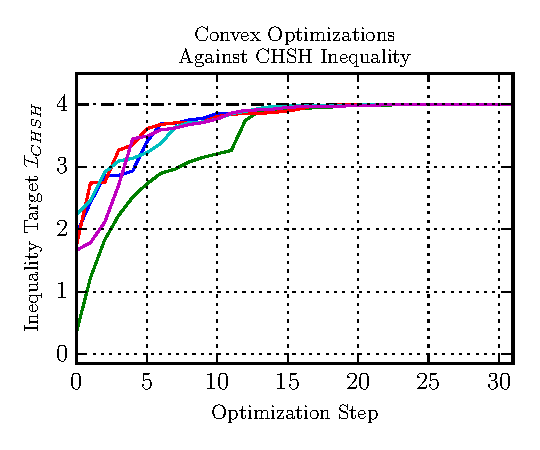
\includegraphics{figures/CHSH_convex.pdf}
            \caption{Convex optimizations against $\mathcal{I}\tsb{CHSH}$ recover algebraic violation of $4$.}
            \label{fig:CHSH_convex}
        \end{minipage}\hspace{0.04\textwidth}%
        \begin{minipage}[b]{.48\textwidth}
            \centering
            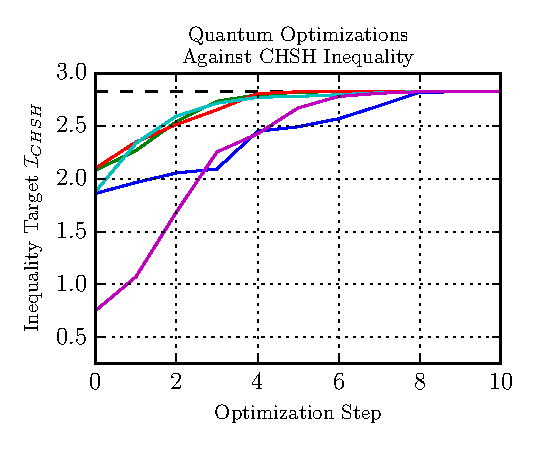
\includegraphics{figures/CHSH_quantum.pdf}
            \caption{Quantum optimizations against $\mathcal{I}\tsb{CHSH}$ recover maximum violation of $2\sqrt{2}$.}
            \label{fig:CHSH_quantum}
        \end{minipage}
    \end{center}
    \end{figure}

    \todo[TC]{Demonstrate Quantum, Convexity}
    \todo[TC]{Why Inequalities are great for optimizations}
    \todo[TC]{Non-linearity}
    \todo[TC]{Techniques Used}
    \todo[TC]{Finding maximum violation of CHSH easily}
    \todo[TC]{Unreliance when number of parameters increases}
    \todo[TC]{Issues with local minimum}
    \todo[TC]{Using initial conditions close to fritz, obtain greater violation}
    \todo[TC]{Greater violation shares possibilistic structure of fritz and violates CHSH under definition}
    \todo[TC]{Not realizable with maximally entangled qubit states}
    \todo[TC]{Not realizable with separable measurements}
    \todo[TC]{Many non-trivial inequalities to be tested}
    \todo[TC]{inequality -> dist -> inequality evolution}
    \section{Conclusions}
    \todo[TC]{Inflation technique allows one to witness fritz incompatibility}
    \todo[TC]{Linear optimization induces certificates which are incompatibility witnesses}
    \todo[TC]{There are quantum distributions in the Triangle Scenario that are incompatible and different from fritz in terms of entanglement but not possibilistic structure}
    \section{Open Questions \& Future Work}
    \todo[TC]{Lots of stuff}
    \appendix
    \section{Computationally Efficient Parametrization of the Unitary Group}
    Spengler, Huber and Hiesmayr \cite{Spengler_2010_Unitary} suggest the parameterization of the unitary group $\mathcal{U}\br{d}$ using a $d\times d$-matrix of real-valued parameters $\lambda_{n, m}$
    \[ U = \bs{\prod_{m=1}^{d-1} \br{\prod_{n=m+1}^{d} \exp\br{i P_n \lambda_{n,m}}\exp\br{i \si_{m,n} \lambda_{m,n}}}} \cdot \bs{\prod_{l=1}^{d} \exp\br{iP_l \lambda_{l,l}}}  \eq \label{eq:spengler_unitary} \]
    Where $P_l$ are one-dimensional projective operators,
    \[ P_l = \ket{l}\bra{l} \eq \label{eq:projective_operator} \]
    and the $\si_{m,n}$ are generalized anti-symmetric $\si$-matrices,
    \[ \sigma_{m,n} = -i \ket{m}\bra{n} +i \ket{n}\bra{m} \]
    Where $1 \leq m < n \leq d$.
    For the sake of reference, let us label the matrix exponential terms in \cref{eq:spengler_unitary} in a manner that corresponds to their affect on an orthonormal basis $\bc{\ket{1}, \ldots, \ket{d}}$.
    \begin{align}
    \begin{split}
        GP_l &= \exp\br{iP_l \lambda_{l,l}} \\
        RP_{n,m} &= \exp\br{i P_n \lambda_{n,m}} \\
        R_{m,n} &= \exp\br{i \si_{m,n} \lambda_{m,n}}
    \end{split} \eq \label{eq:exp_terms}
    \end{align}
    It is possible to remove the reliance on matrix exponential operations in \cref{eq:spengler_unitary} by utilizing the explicit form of the exponential terms in \cref{eq:exp_terms}. As a first step, recognize the defining property of the projective operators \cref{eq:projective_operator},
    \[ P_l^k = \br{\ket{l}\bra{l}}^k = \ket{l}\bra{l} = P_l \]
    This greatly simplifies the global phase terms $GP_l$,
    \[ GP_l = \exp\br{iP_l \lambda_{l,l}} = \sum_{k=0}^{\inf} \f{\br{iP_l \lambda_{l,l}}^k}{k!} = \mathbb{I} + \sum_{k=1}^{\inf} \f{\br{i \lambda_{l,l}}^k}{k!}P_l^k = \mathbb{I} + P_l \bs{\sum_{k=1}^{\inf} \f{\br{i \lambda_{l,l}}^k}{k!}} = \mathbb{I} + P_l \br{e^{i \lambda_{l,l}} - 1} \eq \label{eq:unitary_GP} \]
    Analogously for the relative phase terms $RP_{n,m}$,
    \[ RP_{n,m} = \cdots = \mathbb{I} + P_n \br{e^{i \lambda_{n,m}} - 1} \eq \label{eq:unitary_RP} \]
    Finally, the rotation terms $R_{m,n}$ can also be simplified by examining powers of $i \sigma_{n,m}$,
    \[ R_{m,n} = \exp\br{i \si_{m,n} \lambda_{m,n}} = \sum_{k=0}^{\inf} \f{\br{\ket{m}\bra{n} - \ket{n}\bra{m}}^k \lambda_{m,n}^k}{k!} \]
    One can verify that the following properties hold,
    \begin{align*}
        \br{\ket{m}\bra{n} - \ket{n}\bra{m}}^0 &= \mathbb{I} \\
        \forall k \in \N, k \neq 0 : \br{\ket{m}\bra{n} - \ket{n}\bra{m}}^{2k} &= \br{-1}^k\br{\ket{m}\bra{m} + \ket{n}\bra{n}} \\
        \forall k \in \N : \br{\ket{m}\bra{n} - \ket{n}\bra{m}}^{2k+1} &= \br{-1}^k\br{\ket{m}\bra{n} - \ket{n}\bra{m}}
    \end{align*}
    Revealing the simplified form of $R_{m,n}$,
    \[ R_{m,n} = \mathbb{I} + \br{\ket{m}\bra{m} + \ket{n}\bra{n}} \sum_{j=1}^{\inf} \br{-1}^j\f{\lambda_{n,m}^{2j}}{\br{2j}!} + \br{\ket{m}\bra{n} - \ket{n}\bra{m}} \sum_{j=0}^{\inf} \br{-1}^j\f{\lambda_{n,m}^{2j+1}}{\br{2j+1}!} \]
    \[ R_{m,n} = \mathbb{I} + \br{\ket{m}\bra{m} + \ket{n}\bra{n}} \br{\cos\lambda_{n,m} - 1} + \br{\ket{m}\bra{n} - \ket{n}\bra{m}} \sin\lambda_{n,m} \eq \label{eq:unitary_R} \]
    By combining the optimizations of \cref{eq:unitary_RP,eq:unitary_R,eq:unitary_GP} together we arrive at an equivalent form for \cref{eq:spengler_unitary} that is computational more efficient.
    \[ U = \bs{\prod_{m=1}^{d-1} \br{\prod_{n=m+1}^{d} RP_{n,m}R_{m,n}}} \cdot \bs{\prod_{l=1}^{d} GP_l} \eq \label{eq:fast_spengler_unitary} \]
    \todo[TC]{Explanation of Computational Complexity $\mathcal{O}\br{d^3}$ vs. $\mathcal{O}\br{1}$ using \cite{Moler_2003}}
    \todo[TC]{Pre-Caching for Fixed dimension $d$}

    \section{Parametrization of Quantum States \& Measurements}
    Throughout \cref{sec:optimizations}, we utilize a variety of parameterizations of quantum states and measurements in order to generate quantum-accessible probability distributions. There are numerous techniques that can used when parameterizing quantum states and measurements \cite{Petz_2015, Hedemann_2013,Spengler_2010_Unitary,Fujii_2005,James_2001} with applications \todo[TC]{Finish this sentence}. For our purposes, we need to parameterize the space of quantum-accessible distributions $\prob[\mathcal{Q}]$ that are \textit{realized} on the Triangle Scenario. We have implemented $\prob[\mathcal{Q}]$ under the following description.
    \[ \prob[ABC\mid \rho]\br{abc} = \Tr\bs{\Omega^\intercal \rho \Omega M^{abc}} \defined \Tr\bs{\Omega^\intercal \rho_{AB}\otimes\rho_{BC}\otimes\rho_{CA} \Omega M^a_{A}\otimes M^b_{B} \otimes M^c_{C}} \eq \label{eq:triangle_quantum_distributions} \]

    \subsection{Quantum States}
    The bipartite states $\br{\rho_{AB}, \rho_{BC}, \rho_{CA}}$ of \cref{eq:triangle_quantum_distributions} were taken to be two-qubit density matrices acting on $\Hilb^2 \otimes \Hilb^2$.\footnote{We also considered qutrit $\Hilb^3$ qutit $\Hilb^4$ states. However for $6$ $d$-dimensional $\Hilb^d$ states, the joint density matrix $\rho$ acts on $\br{\Hilb^d}^{\otimes 6}$ making it a $\br{d^6, d^6}$ matrix with $d^{12}$ entries. Computationally only $d = 2$ was feasible for our optimization tasks.} The space of all such states corresponds to the space of all $4\times 4$ positive semi-definite hermitian matrices with unitary trace. There are three distinct techniques that we have considered.

    Taking inspiration from \cite{James_2001}, we can parameterize all such density matrices $\rho$ using \term{Cholesky Parametrization} \cite{Grasmair_2014}. The Cholesky decomposition allows one to write any hermitian positive semi-definite matrix $\rho$ in terms of a lower (or upper) triangular matrix $T$ using $\rho = T^\dagger T$. Our Cholesky parameterization consists of assigning $16$ real-valued parameters $\lambda$ to the entires of $T$ and generating a unitary trace $\rho$ similar to eq. (4.4) of \cite{James_2001}.
    \[ \rho = \f{T^\dagger T}{\Tr\br{T^\dagger T}} \quad T = \pmtrx{\la_{1}&0&0&0\\\la_{2} + i \la_{3}&\la_{4}&0&0\\\la_{5} + i \la_{6}&\la_{7} + i \la_{8}&\la_{9}&0\\\la_{10} + i \la_{11}&\la_{12} + i \la_{13}&\la_{14} + i \la_{15}&\la_{16}} \eq \label{eq:cholesky_param} \]
    Our deviation from exclusiving using \cref{eq:cholesky_param} is two-fold. First, \cref{eq:cholesky_param} is degenerate in that the normalization indicates only $16 - 1 = 15$ parameters are required for fully generic parameterization of all such states $\rho$. Removing this degeneracy is possible although difficult. Second, the parameters $\lambda_i$ carry no physical meaning associated with the state $\rho$, unlike our next parameterization.

    In Spengler, Huber and Hiesmayr's work \cite{Spengler_2010_Unitary}, they discuss how to parameterization density matrices $\rho$ acting on $\Hilb^d$ of rank $k$ through it's spectral decomposition,
    \[ \rho = \sum_{i=1}^{k} p_i \ket{\psi_i}\bra{\psi_i} \quad p_i \geq 0, \sum_{i} p_i = 1, k \leq d \eq \label{eq:unitary_param_density} \]
    Where any orthonormal basis $\bc{\ket{\psi_i}}$ of $\Hilb^d$ can be transformed into a computational basis $\bc{\ket{i}}$ by a unitary $U \in \mathcal{U}\br{d}$ such that $\ket{\psi_i} = U\ket{i}$. We refer to \cref{eq:unitary_param_density} as the \term{Spengler Parametrization}. Without loss of generality we parameterize all full-rank ($k=d$) matrices by simultaneously parameterizing the $d=4$ eigenvalues $p_i$ of \cref{eq:unitary_param_density} using \cref{eq:convex_param} and the unitary group $\mathcal{U}\br{4}$.


    \subsection{Measurements}
    $\Omega$ represents a permutation matrix to be discussed below. $\rho_{AB}$ is the quantum state between party $A$ and $B$ and is represented by a generic density matrix operator acting on $\Hilb^2$

    \subsection{Network Permutation Matrix}

    \section{Convex Parametrization of Finite Probability Distributions}
    As discussed in \cref{sec:optimizations}, there is a need to parameterize the family of all probability distributions $\prob[V]$ over a given set of variables $V = \br{v_1, \ldots, v_{\abs{V}}}$. If the cardinality of $O_{V}$ is finite, then this computationally feasible. The space of probability distributions over $n = \abs{O_{V}}$ distinct outcomes forms a $n-1$ dimensional convex polytope naturally embedded in $\R_{\geq 0}^n$ \cite{Brunner_2013} that is parameterizable by $n-1$ real value parameters; normalization $\sum_{o\bs{V} \in O_V} \prob[V][\outc{V}] = 1$ accounts for the `$-1$'. An example of a non-degenerate parameterization of $\prob[V]$ consists of $n-1$ parameters $\lambda = \br{\lambda_1, \ldots, \lambda_{n-1}}, \lambda_i \in \bs{0, \pi/2}$ which generate the probabilities $n$ probability values $p_j$ using hyperspherical coordinates \cite{Hedemann_2013, Spengler_2010_Unitary},
    \begin{equation}
    \begin{gathered}
        \label{eq:convex_param}
        p_j = \cos^2 \lambda_j \prod_{i=1}^{j-1} \sin^2 \lambda_i \quad \forall j \in 1, \ldots, n - 1 \\
        p_n = \prod_{i=1}^{n-1} \sin^2 \lambda_i
    \end{gathered}
    \end{equation}
    Furthermore due to the periodicity of the parameter space $\lambda$, \cref{eq:convex_param} can be used for either constrained or unconstrained optimization problems.

    Although non-degenerate, this parameterization suffers from uniformity; a randomly sampled vector of parameters $\lambda$ \textit{does not} translate to a randomly sampled probability $\prob[V]$. An easy-to-implement, degenerate parameterization of $\prob[V]$ can be constructed by simply beginning with $n$ real parameters $\lambda = \br{\lambda_1, \ldots, \lambda_n}$, then making them positive and normalized by their sum\footnote{Strictly speaking, \cref{eq:uniform_param} \textit{also} suffers from non-uniformity; being biased toward uniform probability distributions $\prob[V]$. \todo[TC]{Discuss rejection sampling simplex algorithms}}.
    \[ p_j = \f{\abs{\lambda_j}}{\sum_{i=1}^{n} \abs{\lambda_i}} \quad \forall j \in 1, \ldots, n \eq \label{eq:uniform_param} \]
    For various convex optimization tasks sensitive to initial conditions outlined \cref{sec:optimizations}, the latter parameterization of \cref{eq:uniform_param} generally performed better than the former \cref{eq:convex_param}.
    % \nocite{REVTEX41Control}
    % \nocite{apsrev41Control}
    % \bibliographystyle{plain}

    \bibliography{references}
\end{document}